\subsection{Sintetizador de sonidos}
\label{toneGen}

\begin{figure}[H]
	\centering
	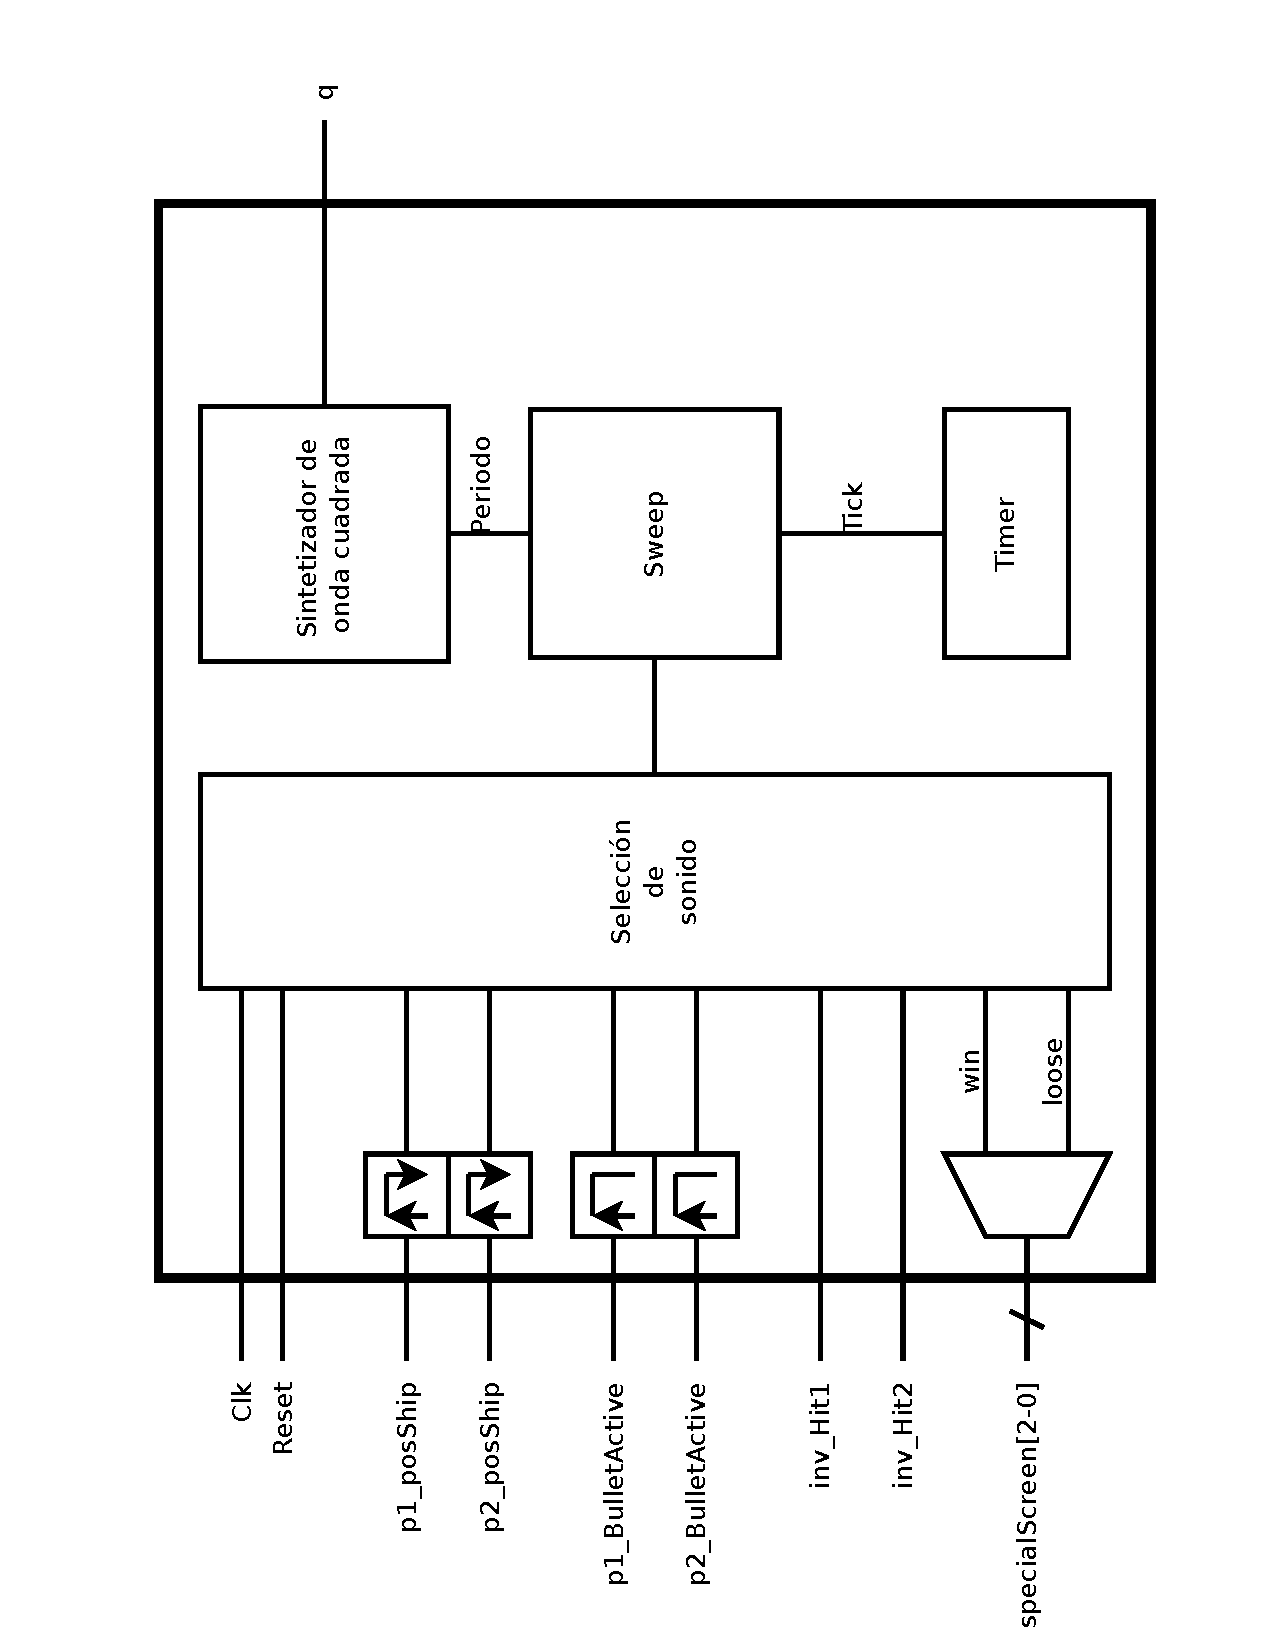
\includegraphics[width=0.65\textwidth, angle=-90] {toneGen_block.pdf}
	\caption{Diagrama de bloques del sintetizador de sonido}\label{fig:toneGen_block}
\end{figure}

Para emular el videojuego original, se ha implementado un sintetizador digital de sonidos que produce melodías que acompañan diferentes acciones del juego: movimiento de la nave, disparo, alcance de invasores y pantallas de victoria y derrota. 

\subsection{Implementación}
Como puede verse en la figura \ref{fig:toneGen_block}, la sintetización del sonido consta de cuatro pasos:

\begin{enumerate}

\item \textbf{Detección de acción}: Para no requerir señales adicionales dentro de la entidad \emph{spaceInvaders}, la detección de acciones se decodifica a través de las señales intermedias \emph{p1\_posShip, p2\_posShip, p1\_BulletActive, p2\_BulletActive, inv\_Hit1, inv\_Hit2} y \emph{specialScreen}, con la ayuda de detectores de flanco y decodificadores.

\item \textbf{Selección de sonido}: Cada sonido del sintetizador se caracteriza por el rango de frecuencias que barre (codificado como \emph{startPeriod} y \emph{endPeriod}). Este bloque selecciona estos valores dependiendo de la acción que da orígen al sonido.

\item \textbf{Barrido de frecuencia}: El rango de frecuencias seleccionado se divide en 32 escalones de 30 ms de duración. En cada instante, este bloque controla la frecuencia a la que oscila el sintetizador de onda cuadrada. 

\item \textbf{Sintetizador de onda cuadrada}: Basado en un temporizador de período regulable, el sintetizador genera una onda cuadrada de ciclo de trabajo 50 \%.

\end{enumerate}

Una vez generada la señal cuadrada, un filtro RC analógico externo limita el ancho de banda a 1 KHz, suavizando la señal y haciendo el sonido menos estridente.

\subsubsection{Testbench}
El testbench comprueba el funcionamiento del sintetizador aislado del resto del videojuego, simulando una de las señales de acción.